\subsection{Workload (product backlog)}
Der laves en product backlog i stedet for en tidplan (se figur \ref{fig:workload}).
\begin{figure}[ht]
	\centering
	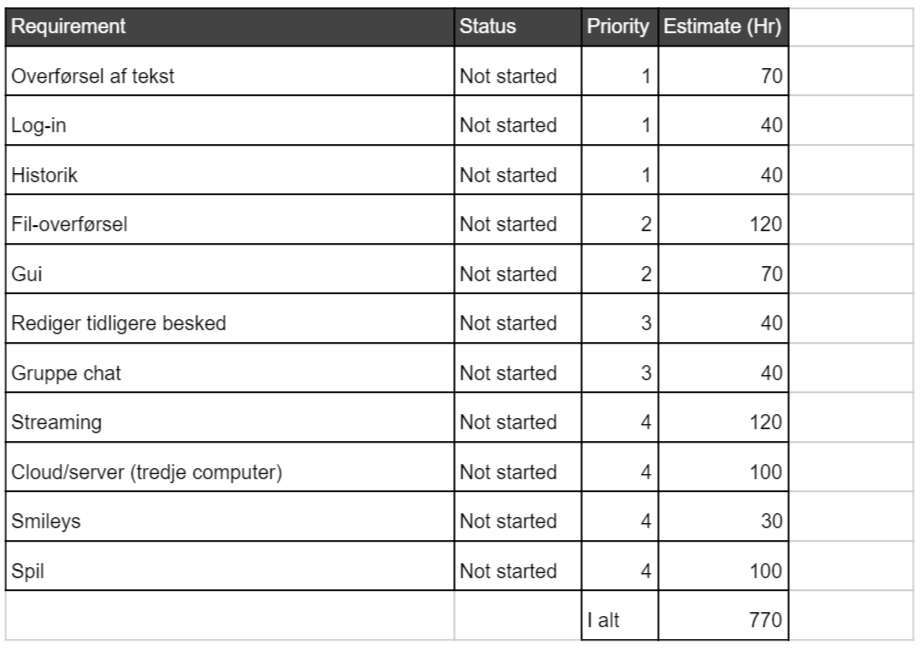
\includegraphics[width=15cm,height=25cm,keepaspectratio]{pictures/Workload.png}
	\caption{Product backlog}
	\label{fig:workload}
	\end{figure}
\newline
En product backlog er et værktøj inden for metoden SCRUM, som viser hvor langt tid en opgaver tager i mandetimer og hvilken status opgaven har (Not started, In process og Finished).
